\NeedsTeXFormat{LaTeX2e}
\documentclass[twocolumn,letterpaper]{igs}
%\documentclass[review,letterpaper]{igs}

\usepackage{stfloats}
\usepackage{verbatim,xspace,amsmath,amssymb,bm}

\usepackage{tikz}
\usetikzlibrary{arrows}

\usepackage{igsnatbib}  % see igs2eguide.tex for example citation styles

\newcommand{\onecol}[1]{\includegraphics[width=86mm]{#1}}
\newcommand{\twocol}[1]{\includegraphics[width=178mm]{#1}}

% math macros
\newcommand\bb{\mathbf{b}}
\newcommand\bc{\mathbf{c}}
\newcommand\bbf{\mathbf{f}}
\newcommand\bn{\mathbf{n}}
\newcommand\bq{\mathbf{q}}
\newcommand\bu{\mathbf{u}}
\newcommand\bv{\mathbf{v}}
\newcommand\by{\mathbf{y}}

\newcommand\bF{\mathbf{F}}
\newcommand\bH{\mathbf{H}}
\newcommand\bQ{\mathbf{Q}}
\newcommand\bV{\mathbf{V}}
\newcommand\bW{\mathbf{W}}
\newcommand\bX{\mathbf{X}}

\newcommand\CC{\mathbb{C}}
\newcommand{\DDt}[1]{\ensuremath{\frac{d #1}{d t}}}
\newcommand{\ddt}[1]{\ensuremath{\frac{\partial #1}{\partial t}}}
\newcommand{\ddx}[1]{\ensuremath{\frac{\partial #1}{\partial x}}}
\newcommand{\ddy}[1]{\ensuremath{\frac{\partial #1}{\partial y}}}
\newcommand{\ddxp}[1]{\ensuremath{\frac{\partial #1}{\partial x'}}}
\newcommand{\ddz}[1]{\ensuremath{\frac{\partial #1}{\partial z}}}
\newcommand{\ddxx}[1]{\ensuremath{\frac{\partial^2 #1}{\partial x^2}}}
\newcommand{\ddyy}[1]{\ensuremath{\frac{\partial^2 #1}{\partial y^2}}}
\newcommand{\ddxy}[1]{\ensuremath{\frac{\partial^2 #1}{\partial x \partial y}}}
\newcommand{\ddzz}[1]{\ensuremath{\frac{\partial^2 #1}{\partial z^2}}}
\newcommand{\Div}{\nabla\cdot}
\newcommand\eps{\epsilon}
\newcommand{\grad}{\nabla}
\newcommand{\ihat}{\mathbf{i}}
\newcommand{\ip}[2]{\ensuremath{\left<#1,#2\right>}}
\newcommand{\jhat}{\mathbf{j}}
\newcommand{\khat}{\mathbf{k}}
\newcommand{\nhat}{\mathbf{n}}
\newcommand\lam{\lambda}
\newcommand\lap{\triangle}
\newcommand\RR{\mathbb{R}}
\newcommand\vf{\varphi}

\newcommand{\Mstar}{$\text{M}^{\bigstar}$\xspace}

\newcommand\alpharight{\alpha_{{}_{\blacktriangleright}}}
\newcommand\alphaup{\alpha_{{\!}_{\blacktriangle}}}

\newcommand{\dxtwo}{\tfrac{\Delta x}{2}}
\newcommand{\dytwo}{\tfrac{\Delta y}{2}}

\newcommand{\half}{\tfrac{1}{2}}


\begin{document}

\title[Stable FVE schemes for the shallow ice approximation]{Stable finite volume element schemes \\ for the shallow ice approximation}

\abstract{The isothermal, non-sliding shallow ice approximation, combined with mass conservation, is a model for ice sheet and glacier flow which determines ice sheet geometry by the solution of a free-boundary problem.  We demonstrate a fully-implicit scheme with no stability restrictions by solving the steady state form of the problem directly, without time-stepping.  First the \cite{Mahaffy1976} finite difference calculation is re-interpreted as a ``finite volume element'' (FVE) scheme so that everywhere-defined numerical fields and a flux integral form of the conservation statement are available in the construction of numerical schemes.  On this FVE basis we build an improved scheme which has both better quadrature in the integral and upwinding on the part of the flux coming from the bed gradient.  The discrete equations are then solved by a parallel Newton scheme which respects the constraint that thicknesses are nonnegative.  The results show superior accuracy to any published results for both flat bed and bedrock-step \citep{JaroschSchoofAnslow2013} exact solutions.  We then apply the improved scheme at 1km resolution to the compute the steady-state geometry of the Greenland ice sheet, using only bedrock elevation and present-day surface mass balance as input data, in a laptop-scale computation.}

\author{Ed Bueler}

\affiliation{Department of Mathematics and Statistics, and Geophysical Institute, University of Alaska Fairbanks, USA \\
E-mail: \emph{\texttt{elbueler\@@alaska.edu}}}

\maketitle

\sectionsize


\section*{Introduction}

The classical finite difference (FD) scheme introduced by \cite{Mahaffy1976} for modeling the Barnes Ice Cap was a first success in modeling ice sheet flow and geometry evolution in two horizontal dimensions.  This scheme numerically solves the shallow ice approximation (SIA; Hutter, 1983)\nocite{Hutter1983} by computing the ice flux at staggered-grid points, using particular choices when evaluating the ice surface slope and thickness.  An advantage of the scheme is its relatively-small stencil, which reduces memory usage in implicit implementations \citep{HindmarshPayne1996,Mahaffy1976} and interprocess communication in parallel implementations \citep{Bueleretal2007}.  Its stability and accuracy properties as an explicit scheme are relatively-well understood in flat-bed cases \citep{Bueleretal2005,HindmarshPayne1996}.  It can also be used as the deformational part of a membrane-stress-resolving hybrid stress balance solution method \citep{BuelerBrown2009}.

Existing numerical schemes for the SIA solve the time-dependent SIA with explicit, semi-implicit, or fully-implicit time-stepping schemes.  All of these have stability restrictions \citep[among others]{Bueleretal2005,EgholmNielsen2010,HindmarshPayne1996,Huybrechtsetal1996,
JaroschSchoofAnslow2013}.  In these applications the SIA is solved with essentially \emph{ad hoc} treatment of the free margin of the ice sheet, for example using projection in explicit schemes to reset computed negative thicknesses back to zero \citep{Bueleretal2005,JaroschSchoofAnslow2013}.

The work of \cite{JouvetBueler2012} is the one exception to the above usage pattern.  They pose and numerically-solve the steady state SIA free boundary problem as a variational inequality \citep{KinderlehrerStampacchia1980} which includes, as an inequality constraint, the fact that ice thickness is never negative.  We follow this idea, by also solving the steady state free boundary problem, but we do so by re-interpreting the well-known Mahaffy method so that it becomes a highly-accurate and scalable scheme.  The new scheme is none-the-less easy to implement because Newton solvers adapted to inequality constraints \citep{BensonMunson2006} are available in the open-source PETSc library \citep{Balayetal2014}.

The classical Mahaffy scheme turns out to be a non-standard quadrature choice in the flux integral which states the conservation of mass.  In this context the integrand, which is the vertically-integrated ice flux in the SIA, is defined everywhere because it comes from a thickness field which lives in a continuous space of trial functions.  These trial functions are piecewise-bilinear on a structured grid of rectangles---i.e.~$Q^1$ finite elements \citep{Elmanetal2005}.  If we think of the method as a ``true'' finite element (FE) method then the test functions we user are piecewise-constant with support on dual rectangular control volumes, so the scheme is a Petrov-Galerkin method \citep{Elmanetal2005}.  But it is more natural to regard the scheme as a ``finite volume element'' \citep[FVE;][]{Cai1990,EwingLinLin2002} method because the weak form we actually use in constructing fully-discrete schemes is simply the flux integral itself, over control volumes, just as would appear in finite volume \citep[FV;][]{LeVeque2002} schemes.  We adopt the FVE terminology because of the greater clarity which comes from regarding the mass conservation equation as being in classical flux-integral form.

Our paper is organized as follows.  We start with a statement of the steady, isothermal SIA model.  We then recall the classical Mahaffy scheme in FD form before re-interpreting it as an FVE scheme and identifying its non-standard midpoint rule application in the flux integral.  Building off this re-interpretation we identify better quadrature in the flux integral, and we then add a bit of first-order upwinding on the part of the flux that comes from the bedrock slope.  The resulting improved scheme, which has the same stencil as the classical Mahaffy scheme, is called ``\Mstar.''  Next we describe the Newton solver which we apply to the discrete equations and constraints.  Results are then given in verification cases, and they are at least as good as those from higher-resolution upwind schemes when applied to the \cite{JaroschSchoofAnslow2013} bedrock-step exact solution.  Then we show how the method is applied to real ice sheets by computing, without time-stepping but at very high resolution, the steady state shape of the Greenland ice sheet in a present-day modeled climate.

In the Appendix we describe how to construct, on certain unstructured finite element triangulations, an analog of the \Mstar improved scheme.


\section*{The continuum model}

The time-dependent evolution equation for the ice thickness $H$ is a mass conservation equation,
\begin{equation}
\frac{\partial H}{\partial t} + \Div \bq = m,  \label{eq:siaevolution}
\end{equation}
where $\bq$ denotes the vertically-integrated flux (units $\text{m}^2/\text{s}$) and $m$ ($\text{m}/\text{s}$) is the surface mass balance, also called the accumulation/ablation function.

The SIA continuum model is the lubrication approximation \citep{Fowler1997} of the Stokes equations for slow-flowing ice, in non-sliding contact with the bed and with a freely-evolving upper surface.  We only consider the isothermal, Glen-power-law \citep{GreveBlatter2009} case.  Let $b$ be the bed and $s = H+b$ the ice surface elevation.  The flux $\bq$ is given by
\begin{equation}
\bq = - \Gamma H^{n+2} |\grad s|^{n-1} \grad s  \label{eq:siaflux}
\end{equation}
where $\Gamma = 2 A (\rho g)^n / (n+2)$ is a positive constant derived from the Glen power $n$, ice softness $A$, ice density $\rho$, and gravity $g$.

The flux $\bq$ has multiple interpretations.  Equations \eqref{eq:siaevolution} and \eqref{eq:siaflux} are often interpreted as a single nonlinear diffusion equation \cite{Huybrechtsetal1996}.  In this case
\begin{equation}
\bq = - D \grad s \quad \text{and} \quad D =  \Gamma H^{n+2} |\grad s|^{n-1}. \label{eq:siafluxdiffusion}
\end{equation}
However, if the bed is not flat then $\grad s$ and $\grad H$ are different.  On the other hand one can compute a vertically-averaged velocity $\bV$, and then treat the flux as arising from the transport of the thickness by $\bV$, that is,
\begin{equation}
\bq = \bV H \quad \text{where} \quad \bV = - \Gamma H^{n+1} |\grad s|^{n-1} \grad s. \label{eq:siafluxvelocity}
\end{equation}
In this case \eqref{eq:siaevolution} is apparently a hyperbolic conservation equation, but this appearance is superficial and deceiving because the velocity depends in part on the gradient of the transported quantity.

The former diffusion interpretation \eqref{eq:siafluxdiffusion} is surely more appropriate in the flat-bed case $b=0$ because in that case \eqref{eq:siaevolution} and \eqref{eq:siaflux} can be transformed to a $p$-Laplacian diffusion equation \citep{Calvoetal2002}.  In general, however, the diffusion-equation interpretation is obscured by the bed gradient $\grad b$ which is in formula \eqref{eq:siafluxdiffusion} for $D$.  This bed gradient is a barrier to theoretical progress on proving the existence and uniqueness of solutions \citep{JouvetBueler2012} and it generates conservation errors at the ice margin in numerical schemes \citep{JaroschSchoofAnslow2013}.

In fact, \cite{JaroschSchoofAnslow2013} propose a third form for the flux, namely
\begin{equation}
   \bq = \boldsymbol{\omega} H^{n+2} \quad \text{where} \quad \boldsymbol{\omega} = - \Gamma |\grad s|^{n-1} \grad s. \label{eq:siafluxjsa}
\end{equation}
The vector field $\boldsymbol{\omega}$ can be thought of as a ``velocity'' which transports $H^{n+2}$, and in this thinking the combination of \eqref{eq:siaevolution} and \eqref{eq:siafluxjsa} becomes a kind of nonlinear hyperbolic equation, but again with a ``velocity'' that actually depends on the gradient of the transported quantity $H$.  However, we will settle on a modification of form \eqref{eq:siafluxjsa}, namely
\begin{equation}
\bq = - D \grad H + \bW H^{n+2},\label{eq:fluxform}
\end{equation}
where $D$ is the same as in \eqref{eq:siafluxdiffusion} and
\begin{equation}
\bW = - \Gamma |\grad s|^{n-1} \grad b.  \label{eq:siaWdefine}
\end{equation}
The vector field $\bW$ can again be thought of as a ``velocity'' which transports $H^{n+2}$, and the combination of \eqref{eq:siaevolution} and \eqref{eq:fluxform} defines a highly-nonlinear diffusion-advection equation.  Note that $\bW=0$ in the case of flat beds, while $\boldsymbol{\omega}$ is both nonzero and diffusive (i.e.~exactly points along $-\grad H$) in that case.

In numerical schemes the advantage of form \eqref{eq:fluxform} over any of \eqref{eq:siafluxdiffusion}, \eqref{eq:siafluxvelocity}, or \eqref{eq:siafluxjsa} is that we can apply a non-oscillatory transport scheme to the ``$\bW H^{n+2}$'' term while preserving accuracy by applying a centered scheme to the diffusive term ``$-D \grad H$''.  The presence of the (often-dominant) leading-order diffusion is also a motivation to use implicit time-stepping, but such implicit schemes also need to determine the location of the free boundary at each time step.

In fact we will only solve the steady-state form of \eqref{eq:siaevolution}, namely
\begin{equation}
\Div \bq = m.  \label{eq:siasteady}
\end{equation}
Though this equation is apparently simpler than \eqref{eq:siaevolution}, it is more difficult to solve in the sense that it is a boundary-value problem wherein the location where the boundary conditions should be applied is unknown \citep{JaroschSchoofAnslow2013,JouvetBueler2012}.  The ice-covered domain where \eqref{eq:siasteady} applies, and the location of the boundary where $\bq=0$, cannot be treated as a small modification of a known boundary in the steady-state problem, while that is the standard approach of time-stepping schemes \citep{Bueleretal2005,Huybrechtsetal1996}.

To be somewhat more precise about boundary conditions, if $m$ is sufficiently-negative near the boundary of $\Omega$ then $H$ reaches zero inside the domain at the free boundary.  At this free boundary, $H\to 0$ and $\bq \to 0$ simultaneously \citep{JouvetBueler2012}.  The problem also has degenerate diffusivity, i.e.~also $D \to 0$ at the free boundary.  Solving equation \eqref{eq:siasteady}, or computing a time-step of \eqref{eq:siaevolution}, as such a free-boundary problem, without a boundary flux applied along any part of the boundary of $\Omega$, is usually called a ``whole'' ice sheet model.  We restrict our attention to such whole ice sheet models.

The problem we solve combines equations \eqref{eq:fluxform} and \eqref{eq:siasteady}, where $D$ and $\bW$ are defined in \eqref{eq:siafluxdiffusion} and \eqref{eq:siaWdefine} respectively.  The input data consists of the bed elevation $b(x,y)$ and the (steady) surface mass balance $m(x,y)$.  Both of these fields are defined on some larger domain $\Omega$ than the ice-covered set, and we assume $m$ sufficiently-negative near the boundary of $\Omega$ so that the ice-covered set is surrounded by a free boundary.  (Alternatively, as in our practical computations, $\Omega$ has no boundary because it is periodic.)  The solution is the nonnegative thickness function $H(x,y)$, and corresponding surface elevation $s(x,y)$.


\section{The classical Mahaffy scheme}   \label{sec:mahaffyfd}

Consider the rectangular structured FD grid, with spacing $\Delta x,\Delta y$, in Figure \ref{fig:fdfemgrids}a.  The \cite{Mahaffy1976} scheme calculates one of the flux components $\bq=(q^x,q^y)$ at the staggered grid points marked by triangles in the Figure.  For these points we introduce notation
\begin{equation}
x_j^\pm = x_j \pm \dxtwo, \qquad y_k^\pm = y_k \pm \dytwo. \label{eq:definexypm}
\end{equation}
At staggered point $(x_j^+,y_k)$ the scheme computes the $x$-component of the flux by
\begin{equation}
q^x_{j+\half,k} = - \Gamma (\hat H_{j+\half,k})^{\,n+2} \alpharight^{\,n-1} \frac{s_{j+1,k} - s_{j,k}}{\Delta x}  \label{eq:mahaffyqx}
\end{equation}
where $s_{j,k} = H_{j,k} + b_{j,k}$ and
\begin{equation}
  \hat H_{j+\half,k} = \frac{H_{j,k} + H_{j+1,k}}{2}.  \label{eq:mahaffyHav}
\end{equation}
The quantity ``$\alpharight$\!'' is an estimate of $|\grad s|$:
\begin{align}
\alpharight^{\,2} &= \left(\frac{s_{j+1,k} - s_{j,k}}{\Delta x}\right)^2  \label{eq:mahaffyalphax} \\
  &\quad + \left(\frac{s_{j,k+1} + s_{j+1,k+1} - s_{j,k-1} - s_{j+1,k-1}}{4 \Delta y}\right)^2. \notag
\end{align}
The formula for the flux $q^y_{j,k+\half}$ at staggered location $(x_j,y_k^+)$, which uses thickness average $\hat H_{j,k+\half}$ and slope estimate $\alphaup$, follows by swapping the roles of $j$ and $k$, and $\Delta x$ and $\Delta y$, in the above equations.

\begin{figure}[ht]
\begin{center}
\begin{tikzpicture}[scale=0.75]
  %uncomment to see grid on which it was generated:
  %\draw[dotted,step=1.0,black,very thin] (0,0) grid (6,4);

  % faint grid
  \draw[gray, dashed] (-0.75,0) -- (6.75,0);
  \draw[gray, dashed] (-0.75,2) -- (6.75,2);
  \draw[gray, dashed] (-0.75,4) -- (6.75,4);
  \draw[gray, dashed] (0,-0.5) -- (0,4.5);
  \draw[gray, dashed] (3,-0.5) -- (3,4.5);
  \draw[gray, dashed] (6,-0.5) -- (6,4.5);

  % regular FD points
  \filldraw (0,0) circle (2.5pt);
  \filldraw (3,0) circle (2.5pt);
  \filldraw (6,0) circle (2.5pt);
  \filldraw (0,2) circle (2.5pt);
  \filldraw (3,2) circle (2.5pt);
  \filldraw (6,2) circle (2.5pt);
  \filldraw (0,4) circle (2.5pt);
  \filldraw (3,4) circle (2.5pt);
  \filldraw (6,4) circle (2.5pt);

  % staggered FD points
  \def\dx{0.12};
  \filldraw (1.5-\dx,2+\dx) -- (1.5+\dx,2) -- (1.5-\dx,2-\dx) -- cycle;
  \filldraw (4.5-\dx,2+\dx) -- (4.5+\dx,2) -- (4.5-\dx,2-\dx) -- cycle;
  \filldraw (3-\dx,1-\dx) -- (3,1+\dx) -- (3+\dx,1-\dx) -- cycle;
  \filldraw (3-\dx,3-\dx) -- (3,3+\dx) -- (3+\dx,3-\dx) -- cycle;

  % dimensions \Delta x, \Delta y
  \draw[latex-latex] (3.2,4.5) -- (5.8,4.5);
  \draw (4.5,5.0) node {$\Delta x$};
  \draw[latex-latex] (6.5,2.2) -- (6.5,3.8);
  \draw (7.0,3) node {$\Delta y$};

  % label center point and dims
  \draw (3,-1.0) node {$x_j$};
  \draw (-1.25,2) node {$y_k$};

  % label as "a"
  \draw (-1.5,5.5) node {{\large a.}};
\end{tikzpicture}
 \quad 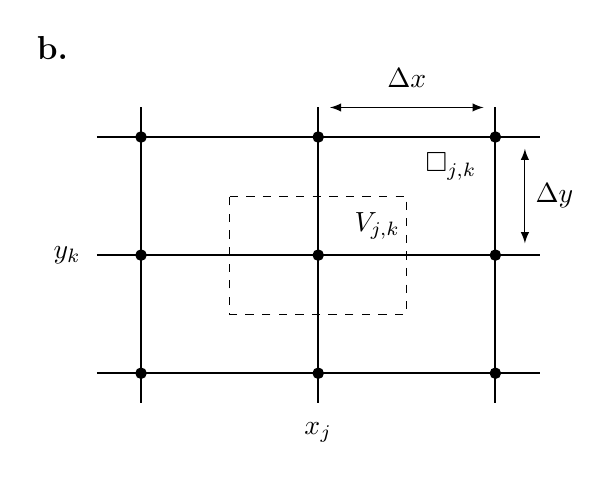
\begin{tikzpicture}[scale=0.75]
  %uncomment to see grid on which it was generated:
  %\draw[dotted,step=1.0,black,very thin] (0,0) grid (6,4);

  % strong grid around elements
  \draw[thick] (-0.75,0) -- (6.75,0);
  \draw[thick] (-0.75,2) -- (6.75,2);
  \draw[thick] (-0.75,4) -- (6.75,4);
  \draw[thick] (0,-0.5) -- (0,4.5);
  \draw[thick] (3,-0.5) -- (3,4.5);
  \draw[thick] (6,-0.5) -- (6,4.5);

  % nodes
  \filldraw (0,0) circle (2.5pt);
  \filldraw (3,0) circle (2.5pt);
  \filldraw (6,0) circle (2.5pt);
  \filldraw (0,2) circle (2.5pt);
  \filldraw (3,2) circle (2.5pt);
  \filldraw (6,2) circle (2.5pt);
  \filldraw (0,4) circle (2.5pt);
  \filldraw (3,4) circle (2.5pt);
  \filldraw (6,4) circle (2.5pt);

  % outline control volume
  \draw[dashed] (1.5,3) -- (4.5,3) -- (4.5,1) -- (1.5,1) -- cycle;

  % label element and control volume
  \draw (5.25,3.5) node {$\square_{j,k}$};
  \draw (4,2.5) node {$V_{j,k}$};

  % dimensions \Delta x, \Delta y
  \draw[latex-latex] (3.2,4.5) -- (5.8,4.5);
  \draw (4.5,5.0) node {$\Delta x$};
  \draw[latex-latex] (6.5,2.2) -- (6.5,3.8);
  \draw (7.0,3) node {$\Delta y$};

  % label center point and dims
  \draw (3,-1.0) node {$x_j$};
  \draw (-1.25,2) node {$y_k$};

  % label as "b"
  \tikzstyle{fontbf} = [font=\bf]
  \draw (-1.5,5.5) node[fontbf] {{\large b.}};
\end{tikzpicture}

\end{center}
\caption{\textbf{a.}~A structured FD grid with regular points (dots) and staggered points (triangles).  \textbf{b.}~The same grid as an FVE grid with rectangular elements $\square_{j,k}$ (solid), nodes (dots), and a dual rectangular control volume $V_{j,k}$ (dashed).  Corners $\ell=0,1,2,3$ of the element are where bases functions $\chi_\ell$ equal one.}
\label{fig:fdfemgrids}
\end{figure}

Slope approximation \eqref{eq:mahaffyalphax} is the least-obvious aspect of the Mahaffy scheme, but the discretization of the mass conservation equation itself is straightforward.  In the steady case the scheme applies centered-difference formulas \citep{MortonMayers2005} to \eqref{eq:siasteady}:
\begin{equation}
\frac{q^x_{j+1/2,k} - q^x_{j-1/2,k}}{\Delta x} + \frac{q^y_{j,k+1/2}- q^y_{j,k-1/2}}{\Delta y} = m_{j,k}.  \label{eq:siasteadyfd}
\end{equation}

Equation \eqref{eq:siasteadyfd}, combined with equations like \eqref{eq:mahaffyqx} for the staggered-grid fluxes, gives one equation in an algebraic system which determines all values $H_{j,k}$ simultaneously.  The algebraic equation coming from \eqref{eq:siasteadyfd} involves the nine unknown values of $H$ at the regular grid points in Figure \ref{fig:fdfemgrids}a.  We call this pattern of dependence the ``stencil'' of the scheme \citep{MortonMayers2005}.


\section{An FVE re-interpretation} \label{sec:fveinterpretation}

The above description of the Mahaffy FD method is familiar to numerical ice sheet modelers, but we now re-derive the scheme from an FE \emph{and} FV perspective.  As Figure \ref{fig:fdfemgrids} suggests, our re-interpretation uses the same structured grid, but the regular grid points $(x_j,y_k)$ are now nodes (degrees of freedom) for a continuous space of trial functions.  The same nodes are also used as centered degrees of freedom for (discontinuous) piecewise-constant test functions, or equivalently as the centers of control volumes over which we compute flux integrals.  The test functions are discontinuous at the FD method's staggered grid points; equivalently the flux integral is over a curve (i.e.~rectangle) which passes through the staggered grid points.  As a ``finite volume element'' (FVE) method we have see discrete conservation, and the construction of upwind-type flux components, just in the standard FV understanding.  However, the FE character remains in that we evaluate an interpolating trial function when computing the flux integral.

We suppose \eqref{eq:siasteady} holds.  By the divergence theorem applied to a subregion $V$ of $\Omega$ we get the flux-integral form of \eqref{eq:siasteady}
\begin{equation}
  \int_{\partial V} \bq \cdot \bn\,ds = \int_V m\, dx\,dy. \label{eq:siaasconservation}
\end{equation}
Here $\partial V$ denotes the boundary of $V$, $\bn$ is the outward normal unit vector, and $ds$ the length element on the closed curve $\partial V$.

An FVE method supposes that the approximation $H^h$ of the thickness solution lies in a finite-dimensional space of continuous functions which are differentiable almost everywhere.  These functions are sufficiently well-behaved so that the approximate flux $\bq^h$ is defined almost everywhere and can be integrated along $\partial V$ in \eqref{eq:siaasconservation}.  But integral equation \eqref{eq:siaasconservation} is only required to hold for a finite set of volumes $V$ which together tile $\Omega$.  This generates a finite system of nonlinear algebraic equations.

Again consider the structured grid of rectangular elements shown in Figure \ref{fig:fdfemgrids}b.  Denote the element with lower-left corner at $(x_j,y_k)$ by $\square_{j,k}$.  When associated with bilinear functions these rectangles are $Q^1$ finite elements \citep{Elmanetal2005}.  A basis for such functions on $\square_{j,k}$ is the set
\begin{equation}
\chi_\ell \left(\frac{x-x_j}{\Delta x},\frac{y-y_k}{\Delta y}\right), \label{eq:elementbasis}
\end{equation}
for $\ell=0,1,2,3$, where
\begin{align*}
\chi_0(\xi,\nu) &= \left(1-\xi\right) \left(1-\nu\right), & \chi_1(\xi,\nu) &= \xi \left(1-\nu\right), \\
\chi_2(\xi,\nu) &= \xi \nu, & \chi_3(\xi,\nu) &= \left(1-\xi\right) \nu.
\end{align*}
With this order, $\chi_\ell=1$ on element corners traversed in counter-clockwise order (Figure \ref{fig:fdfemgrids}b).  Now let
\begin{equation}
S_h = \{u \text{ is bilinear on each $\square_{j,k}$}\}
\end{equation}
be the trial space of continuous functions.  Functions in $S_h$ have a gradient which is defined almost everywhere, but the gradient is discontinuous along the element edges (solid lines in Figure \ref{fig:fdfemgrids}b).

Let $V_{j,k}$ be the control volume with center at $(x_j,y_j)$ (Figure \ref{fig:fdfemgrids}b).  Let
\begin{equation}
S_h^* = \{u \text{ is constant on each $V_{j,k}$}\}
\end{equation}
be the test space of functions which are piecewise constant and discontinuous along the control volume edges (dashed lines in Figure \ref{fig:fdfemgrids}b).

\begin{figure}[ht]
\begin{center}
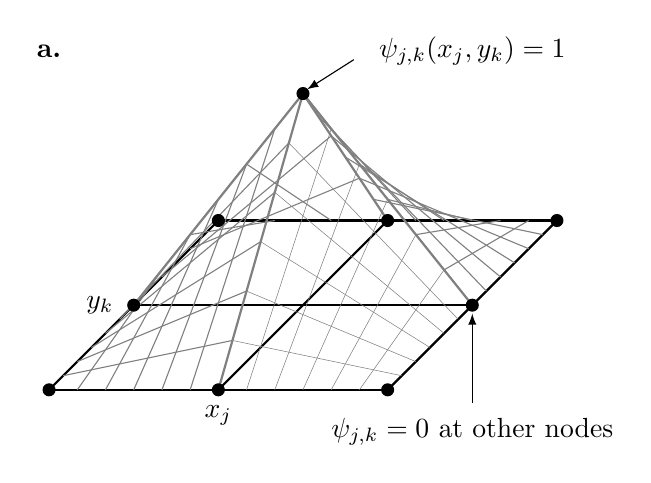
\begin{tikzpicture}[scale=8.6cm/16.0cm]
% min x = 0, max x = 12  so  width = 12 cm, but we pad
% 8.6cm is one-column width for J Glaciol
%\begin{tikzpicture}[scale=0.5]

  % strong grid around elements
  \draw[thick] (0,0) -- (8,0);
  \draw[thick] (2,2) -- (10,2);
  \draw[thick] (4,4) -- (12,4);
  \draw[thick] (0,0) -- (4,4);
  \draw[thick] (4,0) -- (8,4);
  \draw[thick] (8,0) -- (12,4);

  \def\ytop{7};

  % tent lines
  \draw[gray,thick] (6,\ytop) -- (4,0);
  \draw[gray,thick] (6,\ytop) -- (2,2);
  \draw[gray,thick] (6,\ytop) -- (10,2);
  \draw[gray,thick] (6,\ytop) -- (8,4);

  \def\dx{(10.0-6.0)/6};
  \def\dy{(2.0-\ytop)/6};
  \foreach \jj in {1,...,5}
  {
       \draw[gray,very thin] ({6+\jj*\dx},{\ytop+\jj*\dy}) -- ({4+(4/6)*\jj},0.0);
  }

  \def\dx{(4.0-6.0)/6};
  \def\dy{(0.0-\ytop)/6};
  \foreach \jj in {1,...,5}
  {
       \draw[gray,very thin] ({6+\jj*\dx},{\ytop+\jj*\dy}) -- ({10-(2/6)*\jj},{2-(2/6)*\jj});
  }

  \def\dx{(2.0-6.0)/6};
  \def\dy{(2.0-\ytop)/6};
  \foreach \jj in {1,...,5}
  {
       \draw[gray,thin] ({6+\jj*\dx},{\ytop+\jj*\dy}) -- ({4-(4/6)*\jj},0.0);
  }

  \def\dx{(4.0-6.0)/6};
  \def\dy{(0.0-\ytop)/6};
  \foreach \jj in {1,...,5}
  {
       \draw[gray,thin] ({6+\jj*\dx},{\ytop+\jj*\dy}) -- ({2-(2/6)*\jj},{2-(2/6)*\jj});
  }

  \def\dx{(10.0-6.0)/6};
  \def\dy{(2.0-\ytop)/6};
  \foreach \jj in {1,...,5}
  {
       \draw[gray,thin] ({6+\jj*\dx},{\ytop+\jj*\dy}) -- ({8+(4/6)*\jj},4.0);
  }

  \def\dx{(8.0-6.0)/6};
  \def\dy{(4.0-\ytop)/6};
  \foreach \jj in {1,...,5}
  {
       \draw[gray,thin] ({6+\jj*\dx},{\ytop+\jj*\dy}) -- ({10+(2/6)*\jj},{2+(2/6)*\jj});
  }

  \def\dx{(2.0-6.0)/3};
  \def\dy{(2.0-\ytop)/3};
  \foreach \jj in {1,...,2}  % reduce clutter
  {
       \draw[gray,thin] ({6+\jj*\dx},{\ytop+\jj*\dy}) -- ({8-(4/3)*\jj},4.0);
  }

  \def\dx{(8.0-6.0)/3};
  \def\dy{(4.0-\ytop)/3};
  \foreach \jj in {1,...,2}
  {
       \draw[gray,thin] ({6+\jj*\dx},{\ytop+\jj*\dy}) -- ({2+(2/3)*\jj},{2+(2/3)*\jj});
  }

  % nodes in base plane
  \filldraw (0,0) circle (4pt);
  \filldraw (4,0) circle (4pt);
  \filldraw (8,0) circle (4pt);
  \filldraw (2,2) circle (4pt);
  %\filldraw (6,2) circle (4pt);   % (x_j,y_k) is at (6,2)
  \filldraw (10,2) circle (4pt);
  \filldraw (4,4) circle (4pt);
  \filldraw (8,4) circle (4pt);
  \filldraw (12,4) circle (4pt);

  % node at tent top
  \filldraw (6,\ytop) circle (4pt);

  % annotate
  \draw (10,\ytop+1.0) node {$\psi_{j,k}(x_j,y_k)=1$};
  \draw[-latex] (7.2,\ytop+0.8) -- (6.1,\ytop+0.1);
  \draw (10,-1.0) node {$\psi_{j,k}=0$ at other nodes};
  \draw[-latex] (10,-0.3) -- (10,1.8);

  % label center point
  \draw (4,-0.6) node {$x_j$};
  \draw (1.2,2) node {$y_k$};

  % label as "a"
  \tikzstyle{fontbf} = [font=\bf]
  \draw (0,8) node[fontbf] {a.};

\end{tikzpicture}
 \quad 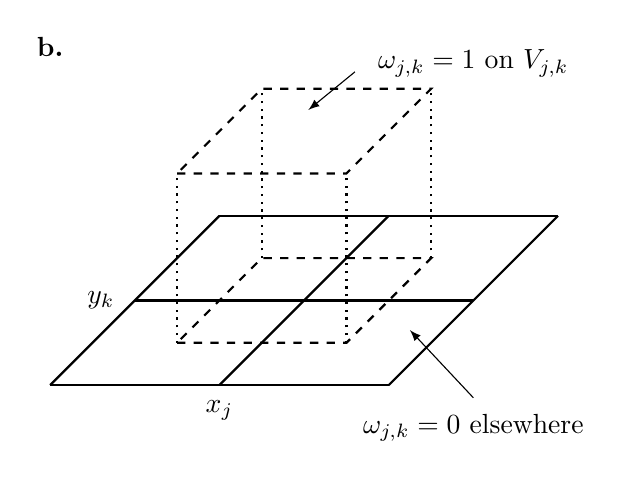
\begin{tikzpicture}[scale=8.6cm/16.0cm]
% min x = 0, max x = 12  so  width = 12 cm, but we pad
% 8.6cm is one-column width for J Glaciol
%\begin{tikzpicture}[scale=0.5]

  % strong grid around elements
  \draw[thick] (0,0) -- (8,0);
  \draw[thick] (2,2) -- (10,2);
  \draw[thick] (4,4) -- (12,4);
  \draw[thick] (0,0) -- (4,4);
  \draw[thick] (4,0) -- (8,4);
  \draw[thick] (8,0) -- (12,4);

  % dashed grid around control volume in base plane
  \draw[thick] (0,0) -- (8,0);

  % label element and control volume
  \def\lift{4};
  \draw[dashed, thick] (3,1) -- (7,1) -- (9,3) -- (5,3) -- cycle;
  \draw[dashed, thick] (3,1+\lift) -- (7,1+\lift) -- (9,3+\lift) -- (5,3+\lift) -- cycle;
  \draw[dotted, thick] (3,1) -- (3,1+\lift);
  \draw[dotted, thick] (7,1) -- (7,1+\lift);
  \draw[dotted, thick] (9,3) -- (9,3+\lift);
  \draw[dotted, thick] (5,3) -- (5,3+\lift);

  % annotate
  \draw (10,\lift+3.6) node {$\omega_{j,k}=1$ on $V_{j,k}$};
  \draw[-latex] (7.2,\lift+3.4) -- (6.1,\lift+2.5);
  \draw (10,-1.0) node {$\omega_{j,k}=0$ elsewhere};
  \draw[-latex] (10,-0.3) -- (8.5,1.3);

  % label center point
  \draw (4,-0.6) node {$x_j$};
  \draw (1.2,2) node {$y_k$};

  % label as "b"
  \tikzstyle{fontbf} = [font=\bf]
  \draw (0,8) node[fontbf] {b.};

\end{tikzpicture}

\end{center}
\caption{\textbf{a.}~A continuous ``hat'' basis function $\psi_{j,k}(x,y)$ in the trial space $S_h$.  \textbf{b.}~A discontinuous, piecewise-constant basis function $\omega_{j,k}(x,y)$ in the test space $S_h^*$.}
\label{fig:fembases}
\end{figure}

Bases of $S_h$ and $S_h^*$ are formed by those functions which take value one at a single node, and zero at all other nodes.  By definition, $\psi_{j,k}(x,y)$ is the unique function in $S_h$ so that $\psi_{j,k}(x_r,y_s) = \delta_{jr} \delta_{ks}$, while $\omega_{j,k}(x,y)$ is the unique function in $S_h^*$ so that $\omega_{j,k}(x_r,y_s) = \delta_{jr} \delta_{ks}$; see Figure \ref{fig:fembases}.  We will use a periodic grid with $N_x$ rectangles in the $x$-direction and $N_y$ in the $y$ direction, so there are $N=N_xN_y$ distinct nodes and $\dim S_h = \dim S_h^* = N$.  

We seek an approximate solution $H^h$ from $S_h$.  Let $b^h$ be the piecewise-bilinear interpolant of the bed elevation $b$, and let $s^h=H^h+b^h$; both are in $S_h$.  We denote by $\bq^h$ the flux computed from formula \eqref{eq:siaflux} using $H^h$ and $b^h$, so $\bq^h$ is well-defined on the interior of each element.  We require \eqref{eq:siaasconservation} to hold for this $\bq^h$ and all volumes $V_{j,k}$.  This is, however, equivalent to multiplying \eqref{eq:siasteady} by $\omega_{j,k}$ and then integrating by parts, though such a calculation requires the generalized-function idea that the derivative of a step function is a Dirac delta function.

Both the classical Mahaffy scheme, and our improved scheme below, assume midpoint quadrature on the right-hand integral in \eqref{eq:siaasconservation}.  Thus we seek $H^h$ in $S_h$ satisfying
\begin{equation}
  \int_{\partial V_{j,k}} \bq^h \cdot \bn\,ds = m_{j,k}\, \Delta x \Delta y, \label{eq:siafve}
\end{equation}
for all $j,k$.  This will give a finite algebraic system once we choose a quadrature rule on the left.

We decompose the integral in \eqref{eq:siafve} into the four edges which form $\partial V_{j,k}$:
\begin{align}
\int_{\partial V_{j,k}} \bq^h \cdot \bn\,ds &= \int_{y_k^-}^{y_k^+} q^x(x_j^+,y)\,dy \label{eq:fluxintdecomp} \\
&\quad + \int_{x_j^-}^{x_j^+} q^y(x,y_k^+)\,dx \notag \\
&\quad - \int_{y_k^-}^{y_k^+} q^x(x_j^-,y)\,dy \notag \\
&\quad - \int_{x_j^-}^{x_j^+} q^y(x,y_k^-)\,dx. \notag
\end{align}
Though $\bq^h$ is a well-defined, bounded function, it is discontinuous across element boundaries.  For example, in the first integral on the right in \eqref{eq:fluxintdecomp} the integrand $f(y) = q^x(x_j^+,y)$ has a jump discontinuity at the midpoint $y=y_k$ of the interval of integration because $s^h_y$ is discontinuous there.  On the other hand, formula \eqref{eq:mahaffyqx} in the Mahaffy FD scheme computes the normal component of $\bq^h$ at the center of the right edge of the control volume shown in Figure \ref{fig:fdfemgrids}b, that is, at $y=y_k$.

In fact the Mahaffy scheme computes each integral in \eqref{eq:fluxintdecomp} by the midpoint method, but by \emph{averaging the discontinuous component of the surface gradient across its jump discontinuity}.  Thus Mahaffy does not use a true quadrature, because the integrand $\bq^h\cdot \bn$ does not have a value at the quadrature point.

To turn this idea into formulas, observe that the thickness $H^h$ and the $x$-derivative $\partial s^h/\partial x = s^h_x$ are continuous along the edge between elements $\square_{j,k}$ and $\square_{j,k-1}$.  Indeed, using the element basis \eqref{eq:elementbasis} the surface gradient on $\square_{j,k}$ has components
\begin{align}
s^h_x(x,y) &= \frac{s_{j+1,k}-s_{j,k}}{\Delta x} \left(1-\frac{y-y_k}{\Delta y}\right)  \label{eq:grads} \\
   &\quad + \frac{s_{j+1,k+1}-s_{j,k+1}}{\Delta x} \left(\frac{y-y_k}{\Delta y}\right), \notag \\
s^h_y(x,y) &= \frac{s_{j,k+1}-s_{j,k}}{\Delta y} \left(1-\frac{x-x_j}{\Delta x}\right) \notag \\
   &\quad + \frac{s_{j+1,k+1}-s_{j+1,k}}{\Delta y} \left(\frac{x-x_j}{\Delta x}\right). \notag
\end{align}
The same functions on $\square_{j,k-1}$ can be calculated by shifting the index $k$ to $k-1$.  Thus the continuous function $s^h_x(x,y)$ has value
\begin{equation}
s^h_x(x_j^+,y_k) = \frac{s_{j+1,k}-s_{j,k}}{\Delta x} \label{eq:femsxstag}
\end{equation}
at the midpoint in the first integral in \eqref{eq:fluxintdecomp}.  Similarly, writing-out $H^h(x,y)$ using the element basis \eqref{eq:elementbasis} gives
\begin{equation}
H^h(x_j^+,y_k) = \frac{H_{j,k}+H_{j+1,k}}{2} \label{eq:femHstag}
\end{equation}
at the midpoint, which is \eqref{eq:mahaffyHav}.  But the $y$-derivative $\partial s^h/\partial y = s^h_y$ has different values above (on $\square_{j,k}$) and below (on $\square_{j,k-1}$) the element boundary at $y = y_k$; the limits are:
\begin{align}
s^h_y(x_j^+,y_k\!+\!0) = \frac{s_{j,k+1}-s_{j,k} + s_{j+1,k+1}-s_{j+1,k}}{2\Delta y}, \\
s^h_y(x_j^+,y_k\!-\!0) = \frac{s_{j,k}-s_{j,k-1} + s_{j+1,k}-s_{j+1,k-1}}{2\Delta y}. \notag
\end{align}
The average of these values is not a value of $s_y^h$, but a re-construction thereof:
\begin{equation}
\widehat{s^h_y}(x_j^+,y_k) = \frac{s_{j,k+1} + s_{j+1,k+1} - s_{j,k-1} - s_{j+1,k-1}}{4\Delta y}. \label{eq:femsystagcrime}
\end{equation}
Formula \eqref{eq:femsystagcrime} is exactly the estimate of $\partial s/\partial y$ which appears in FD formula \eqref{eq:mahaffyalphax}.

In our FVE interpretation, the Mahaffy scheme uses \eqref{eq:femsxstag}, \eqref{eq:femHstag}, and \eqref{eq:femsystagcrime} in the midpoint rule:
\begin{align}
&\int_{y_k^-}^{y_k^+} q^x(x_j^+,y)\,dy  \label{eq:femmahaffyfirstint} \\
  &\quad\approx - \Delta y\, \Gamma H^h(x_j^+,y_k)^{n+2} \,\alpharight^{\,(n-1)/2} s^h_x(x_j^+,y_k). \notag 
\end{align}
where
\begin{equation}
\alpharight^2 = s^h_x(x_j^+,y_k)^2 + \widehat{s^h_y}(x_j^+,y_k)^2
\end{equation}
is the same as in \eqref{eq:mahaffyalphax}.

Mahaffy thus approximates each integral on the right in \eqref{eq:fluxintdecomp} by a perfectly-reasonable quadrature ``crime'' \citep[compare][]{Strang1972} which uses averaging across a discontinuity to reconstruct a slope.  Equation \eqref{eq:femmahaffyfirstint}, and the corresponding approximations of the other integrals in \eqref{eq:fluxintdecomp}, gives the same approximations of the fluxes as \eqref{eq:mahaffyqx} and \eqref{eq:mahaffyalphax} at staggered points $(x_j^\pm,y_k)$ and $(x_j,y_k^\pm)$.  By using these approximate fluxes to compute the integrals in equation \eqref{eq:fluxintdecomp}, and dividing equation \eqref{eq:siafve} by control volume area $\Delta x\,\Delta y$, we get FD equation \eqref{eq:siasteadyfd}.


\section{An improved scheme}  \label{sec:star}

We now return to the goal of accurately-generating an algebraic equation from \eqref{eq:siafve} by quadrature along $\partial V_{j,k}$.  From this point of view it is easy to improve upon the Mahaffy technique, and we do so.  We also use flux decomposition \eqref{eq:fluxform} with an upwind-type discretization on $\bW H^{n+2}$, because $\bW$ is proportional to the bed gradient $\grad b$.  Together these improvements define the ``\Mstar'' scheme.

Because $H^h$ and $b^h$ live in the space of continuous piecewise-bilinear functions $S_h$, the numerical approximation $\bq^h$ from formula \eqref{eq:siaflux} is defined and smooth on the interior of each element, but $\bq^h$ is discontinuous across the element boundaries.  So now we break each interval of integration on the right side of \eqref{eq:fluxintdecomp} into two parts and use the midpoint rule, the optimal one-point rule, on each half.  For example, we break the first integral at $y=y_k$:
\begin{align}
&\int_{y_k^-}^{y_k^+} q^x(x_j^+,y)\,dy  \label{eq:starbreakfirst} \\
  &\quad= \int_{y_k^-}^{y_k} q^x(x_j^+,y)\,dy + \int_{y_k}^{y_k^+} q^x(x_j^+,y)\,dy \notag \\
  &\quad\approx \frac{\Delta y}{2} \left(q^x(x_j^+,y_k-\tfrac{\Delta y}{4}) + q^x(x_j^+,y_k+\tfrac{\Delta y}{4})\right). \notag
\end{align}
Recalling notation \eqref{eq:definexypm}, we see that values $q^x(x_j^+,y_k\pm\tfrac{\Delta y}{4})$ are simply evaluations of $\bq^h$ at points of continuity: $(x_j^+,y_k+\tfrac{\Delta y}{4})$ is inside element $\square_{j,k}$ while $(x_j^+,y_k-\tfrac{\Delta y}{4})$ is inside $\square_{j,k-1}$.  Similar formulas to \eqref{eq:starbreakfirst} apply to the other three integrals on the right side of \eqref{eq:fluxintdecomp}.

Figure \ref{fig:improvequadrature} shows all eight quadrature points needed to compute the full integral over $\partial V_{j,k}$ in \eqref{eq:siafve}.  At each quadrature point we evaluate the $x$- or $y$-component of $\bq^h$ and then multiply by a constant to get the appropriate integral.  Thus we can write our approximation of \eqref{eq:siafve} as
\begin{equation}
\sum_{s=0}^7 \bc_s \cdot \bq^h(x_j^s,y_k^s) = m_{j,k}\,\Delta x\,\Delta y  \label{eq:siamstar}
\end{equation}
where
\begin{align}
\bc_0 &= \bc_7 = \left(0, \tfrac{\Delta y}{2}\right),  \label{eq:cs} \\
\bc_1 &= \bc_2 = \left(\tfrac{\Delta x}{2},0\right),  \notag \\
\bc_3 &= \bc_4 = \left(0, -\tfrac{\Delta y}{2}\right),  \notag \\
\bc_5 &= \bc_6 = \left(-\tfrac{\Delta x}{2},0\right),  \notag
\end{align}
and
\begin{align}
x_j^0 &= x_j^7 = x_j + \tfrac{\Delta x}{2}, & y_k^1 &= y_k^2 = y_k + \tfrac{\Delta y}{2}, \label{eq:xjsyks} \\
x_j^1 &= x_j^6 = x_j + \tfrac{\Delta x}{4}, & y_k^0 &= y_k^3 = y_k + \tfrac{\Delta y}{4}, \notag \\
x_j^2 &= x_j^5 = x_j - \tfrac{\Delta x}{4}, & y_k^4 &= y_k^7 = y_k - \tfrac{\Delta y}{4}, \notag \\
x_j^3 &= x_j^4 = x_j - \tfrac{\Delta x}{2}, & y_k^5 &= y_k^6 = y_k - \tfrac{\Delta y}{2}. \notag
\end{align}

Clearly, implementing equation \eqref{eq:siamstar} requires evaluating the piecewise-bilinear function $\bq^h(x,y)$ at a given quadrature point, which means finding the correct element from the indices $s,x,y$.  Let $\eta(t)$ be the Heaviside step function, so that $\eta(t)=0$ if $t<0$ and $\eta(t)=1$ if $t>0$.  In our indexing, point $(x_j^s,y_k^s)$ is in element $\square_{u,v}$ if and only if $u = j-\eta(x_j^s-x_j)$ and $v=k-\eta(y_k^s-y_k)$.

\begin{figure}[ht]
\begin{center}
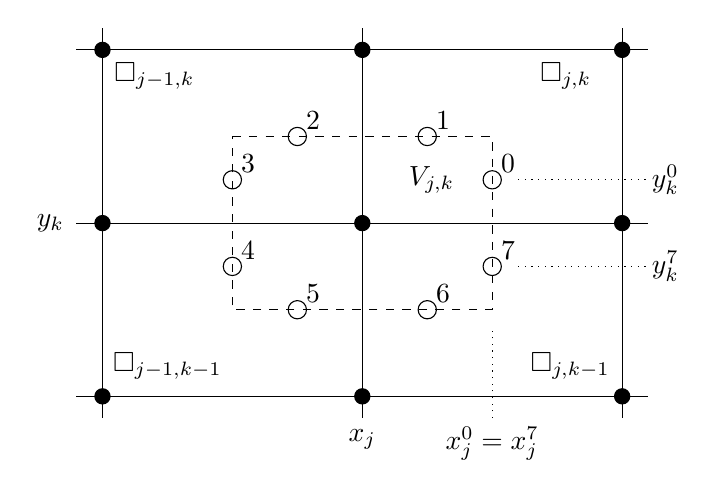
\begin{tikzpicture}[scale=1.1]
  %uncomment to see grid on which it was generated:
  %\draw[dotted,step=1.0,black,very thin] (0,0) grid (6,4);

  % strong grid around elements
  \draw (-0.3,0) -- (6.3,0);
  \draw (-0.3,2) -- (6.3,2);
  \draw (-0.3,4) -- (6.3,4);
  \draw (0,-0.25) -- (0,4.25);
  \draw (3,-0.25) -- (3,4.25);
  \draw (6,-0.25) -- (6,4.25);

  % nodes
  \filldraw (0,0) circle (2.5pt);
  \filldraw (3,0) circle (2.5pt);
  \filldraw (6,0) circle (2.5pt);
  \filldraw (0,2) circle (2.5pt);
  \filldraw (3,2) circle (2.5pt);
  \filldraw (6,2) circle (2.5pt);
  \filldraw (0,4) circle (2.5pt);
  \filldraw (3,4) circle (2.5pt);
  \filldraw (6,4) circle (2.5pt);

  % outline control volume
  \draw[dashed] (1.5,3) -- (4.5,3) -- (4.5,1) -- (1.5,1) -- cycle;

  % mark quadrature points

  \draw (4.5,2.5) circle (3.0pt) node[shift={(0.2,0.2)}] {0};
  \draw (3.75,3)  circle (3.0pt) node[shift={(0.2,0.2)}] {1};
  \draw (2.25,3)  circle (3.0pt) node[shift={(0.2,0.2)}] {2};
  \draw (1.5,2.5) circle (3.0pt) node[shift={(0.2,0.2)}] {3};
  \draw (1.5,1.5) circle (3.0pt) node[shift={(0.2,0.2)}] {4};
  \draw (2.25,1)  circle (3.0pt) node[shift={(0.2,0.2)}] {5};
  \draw (3.75,1)  circle (3.0pt) node[shift={(0.2,0.2)}] {6};
  \draw (4.5,1.5) circle (3.0pt) node[shift={(0.2,0.2)}] {7};

  % label elements and control volume
  \draw (3.8,2.5) node {$V_{j,k}$};
  \draw (5.35,3.7) node {$\square_{j,k}$};
  \draw (5.4,0.35) node {$\square_{j,k-1}$};
  \draw (0.6,3.7) node {$\square_{j-1,k}$};
  \draw (0.75,0.35) node {$\square_{j-1,k-1}$};

  % label center point
  \draw (3,-0.5) node {$x_j$};
  \draw (-0.6,2) node {$y_k$};

  % indicate coordinates of quadrature points
  \draw[dotted] (4.5,-0.25) -- (4.5, 0.8);
  \draw (4.5,-0.55) node {$x_j^0=x_j^7$};
  \draw[dotted] (4.8,2.5) -- (6.3, 2.5);
  \draw (6.5,2.5) node {$y_k^0$};
  \draw[dotted] (4.8,1.5) -- (6.3, 1.5);
  \draw (6.5,1.5) node {$y_k^7$};

\end{tikzpicture}

\end{center}
\caption{For equation \eqref{eq:siamstar} we evaluate $\bq^h(x,y)$ at eight quadrature points (numbered circles) along $\partial V_{j,k}$ (dashed).}
\label{fig:improvequadrature}
\end{figure}

The number of flux-evaluations for the improved method is twice that for the classical method, but the stencils are the same because the algebraic equation for the point $(x_j,y_k)$ uses the same nine nodal values of $H^h$.  (In fact both the improved and classical methods evaluate $\bq^h(x,y)$ at only four locations \emph{in each element}, the former at the midpoint of every side of every element.)

Eight half-edges make up $\partial V_{j,k}$, with each half-edge inside an element.  Thus one could propose further-improved quadrature, replacing the midpoint rule by higher-order methods (e.g.~2-point Gauss-Legendre).  Also, the $Q^1$ elements here could be replaced by higher-order $Q^2$ elements.  Though such methods have not been tested, even in the flat bed case the largest numerical SIA errors occur near the free boundary (margin) where the exact solution $H$ has low regularity \citep{Bueleretal2005}.  Thus higher-order quadrature and interpolation degree will probably not give much advantage.  Our improved method represents a measurable accuracy and Newton-method-convergence improvement over the classical Mahaffy method---see Results section---primarily because the improved method evaluates the flux approximation $\bq^h$ at points of continuity, not because the order of quadrature or interpolation is flawed in the classical scheme.

\cite{JaroschSchoofAnslow2013} show that the Mahaffy scheme can suffer from significant mass conservation errors at locations of abrupt change in the bed elevation, even away from the free boundary.  (I.e.~even with positive thickness at all involved grid points.)  In such cases, when the bed gradient dominates the thickness gradient, the mass conservation equation has ``hyperbolic'' character.  They implement a high-resolution upwind scheme \citep{LeVeque2002} based on flux form \eqref{eq:siafluxjsa}, and they show it reduces error such mass conservation errors, in the sense of giving numerical results which are close in volume to an exact solution (see Results section).  Their upwinding scheme expands the stencil, however, so that computing $\bq$ at point $(x_j,y_k)$ involves thickness $H_{j+2,k}$, two cells away, and they use explicit time-stepping.  Compare to theirs, we propose an implicit (see next section), first-order form of upwinding, and we use their bedrock-step exact solution for testing our scheme (Results section).  For our implicit solution method, upwinding is not required for stability or non-oscillation.

Form \eqref{eq:fluxform} decomposes the flux $\bq$ into a diffusion part and a transport part.  We denote the transport part by $\tilde \bq = \bW H^{n+2}$, where $\bW$ is computed by formula \eqref{eq:siaWdefine}.  So far we have evaluated the whole flux $\bq$ at each quadrature point, but we propose to upwind $\tilde \bq$ by changing the location where $H^{n+2}$ is evaluated according to the direction of $\bW$.  Evaluation of $D\grad H$ and $\bW$ is unchanged.

For example, the upwind modification at $(x_j^0,y_k^0)$ uses the sign of
\begin{equation}
W^x_* = W^x(x_j^0,y_k^0),
\end{equation}
where $\bW=(W^x,W^y)$.  Based on this value we shift the evaluation of $H$ in $\tilde \bq$ upwind by a quarter of an element width:
\begin{align}
&\tilde \bq^x(x_j^0,y_k^0)  \label{eq:upwindschemex} \\
&\quad = W^x_* \begin{cases}
                 H(x_j+\tfrac{\Delta x}{4},y_k^0)^{n+2}, & W^x_* \ge 0, \\
                 H(x_j+\tfrac{3\Delta x}{4},y_k^0)^{n+2}, & W^x_* < 0.
             \end{cases} \notag
\end{align}
Note $\operatorname{sgn}\, W^x_*=-\operatorname{sgn} b^x(x_j^0,y_k^0)$, where $\grad b = (b^x,b^y)$.  These upwind modifications are shown by horizontal arrows in Figure \ref{fig:upwindterm}.  Upwinding at the other seven points along $\partial V_{j,k}$ (Figure \ref{fig:improvequadrature}) is achieved by similar formulas.

\begin{figure}[ht]
\begin{center}
\begin{tikzpicture}[scale=1.8]
  %uncomment to see grid on which it was generated:
  %\draw[dotted,step=1.0,black,very thin] (0,0) grid (6,4);

  % strong grid around elements
  \draw (-0.3,0) -- (3.3,0);
  \draw (-0.3,2) -- (3.3,2);
  \draw (0,-0.3) -- (0,2.3);
  \draw (3,-0.3) -- (3,2.3);

  % nodes
  \filldraw (0,0) circle (1.5pt);
  \filldraw (3,0) circle (1.5pt);
  \filldraw (0,2) circle (1.5pt);
  \filldraw (3,2) circle (1.5pt);

  % outline control volume
  \draw[dashed, thick] (-0.25,1) -- (1.5,1) -- (1.5,-0.25);

  % mark quadrature points
  \draw (1.5,0.5)  circle (2.0pt);
  \draw (0.75,1.0) circle (2.0pt);

  % mark upwind points
  \draw (1.125,0.5) node {$+$};
  \draw (1.875,0.5) node {$+$};
  \draw (0.75,0.75) node {$+$};
  \draw (0.75,1.25) node {$+$};

  % arrows to suggest upwinding
  %\draw[-latex] (1.6,0.4) -- (1.80,0.4);
  %\draw[-latex] (1.4,0.4) -- (1.20,0.4);
  %\draw[-latex] (0.65,1.05) -- (0.65,1.2);
  %\draw[-latex] (0.65,0.95) -- (0.65,0.8);

  % label elements and control volume
  \draw (2.7,1.7) node {$\square_{j,k}$};

  % label lower-left corner
  \draw (0,-0.5) node {$x_j$};
  \draw (-0.5,0) node {$y_k$};

  % indicate coordinates of quadrature point
  \draw (1.5,-0.5) node {$x_j^0$};
  \draw[dotted] (2.8,0.5) -- (3.2, 0.5);
  \draw (3.4,0.52) node {$y_k^0$};

\end{tikzpicture}

\end{center}
\caption{On element $\square_{j,k}$, when computing the flux at quadrature points $0$ and $1$ (circles), upwinding of the flux term $\tilde \bq = \bW H^{n+2}$ evaluates the thicknesses $H$ at locations shown with ``$+$'', according to the sign of the components of $\bW$.}
\label{fig:upwindterm}
\end{figure}

This form of upwinding, which does not expand the stencil, is most important at locations of low regularity of the solution, and we will see in verification that it achieves higher accuracy than both the apparently second-order Mahaffy scheme and the reported results for the higher-resolution explicit scheme of \citep{JaroschSchoofAnslow2013}.

We call the method which combines both improvements (quadrature and upwinding) the ``\Mstar'' method.  The convergence of the Newton method for solving the system of constrained nonlinear algebraic equations is greatly improved for real ice sheet geometries over the classical Mahaffy scheme.


\section{Solution of the equations} \label{sec:solution}

We can now write down a system of nonlinear algebraic equations, but it remains to describe the numerical solution of this system.  This is nontrivial because we solve for steady state directly, and because numerically-locating the free boundary (ice sheet margin) is an integral part of the problem.  We suppose from now on that the structured grid has periodic boundary conditions (b.c.s), as appropriate to a whole ice sheet model.

Each equation in the \Mstar scheme is simply \eqref{eq:siamstar}, with upwind modification \eqref{eq:upwindschemex} used when evaluating the flux.  The resulting highly-nonlinear system of $N=N_x N_y$ equations
\begin{equation}
F_{j,k}(\bH) = 0   \label{eq:nonlinsystem}
\end{equation}
is supposed to determine $N$ unknowns, a vector $\bH=\{H_{j,k}\}$; note ``$H^h(x,y)$'' and ``$\bH$'' are two notations for the same discrete thickness representation.  However, system \eqref{eq:nonlinsystem} is not, by itself, an adequate description because each unknown is constrained by the obvious fact that thicknesses are nonnegative numbers.  We write
\begin{equation}
\bH \ge 0,  \label{eq:nonlinconstraints}
\end{equation}
meaning that each component of the vector is nonnegative.  Requirements \eqref{eq:nonlinsystem} and \eqref{eq:nonlinconstraints} can be combined into a variational inequality \citep{JouvetBueler2012,KinderlehrerStampacchia1980}.  Equivalently, we can write them as a complementarity problem \citep{BensonMunson2006}:
\begin{equation}
\bH \ge 0, \quad \bF(\bH) \ge 0, \quad \bH \cdot \bF(\bH) = 0.  \label{eq:nonlincomplementarity}
\end{equation}

We solve \eqref{eq:nonlinsystem} and \eqref{eq:nonlinconstraints} by a ``constrained'' Newton solver, specifically by the reduced-set method \citep{BensonMunson2006} implemented in PETSc \citep{Balayetal2014}.  The open-source C code used in the current paper\footnote{Clone the repository at \begin{center}\texttt{https://github.com/bueler/sia-fve}\end{center}  See \texttt{README.md} in directory \texttt{petsc/} to compile \texttt{mahaffy.c} and run the examples.  The residual-evaluating method in \texttt{mahaffy.c} is called \texttt{FormFunctionLocal()}.} is surprisingly brief because its only non-trivial part is a ``residual'' subroutine which records the equations \eqref{eq:nonlinsystem} themselves.  The Jacobian of system \eqref{eq:nonlinsystem}, i.e.~the $N\times N$ matrix
\begin{equation}
J = \left(\,\frac{\partial F_{j,k}}{\partial H_{r,s}}\,\right),
\end{equation}
is computed automatically and numerically within PETSc by finite-differencing \citep{Kelley2003}.  Numerical Jacobian evaluation is made efficient by ``coloring'' the nodes so that only nine evaluations of the residual are needed to compute the finite-difference derivatives \citep{CurtisPowellReid1974}.  Because of periodicity and the coloring algorithm, the grid dimensions $N_x$ and $N_y$ must be divisible by three.

A Newton solver requires an initial iterate $H^{(0)}$, for which we give a heuristic which seems to work well for both ice sheet and glacier scale problems.  From the steady surface mass balance data $m_{j,k}$, in meters per year, we compute
\begin{equation}
H_{j,k}^{(0)} = \big(1000.0\,m_{j,k}\big)_+  \label{eq:nonlininitialheuristic}
\end{equation}
where $x_+ = \max\{0,x\}$.  In other words, we build the initial iterate by simply piling up one thousand years of accumulation, without flow.

Additionally we apply a simple ``parameter continuation'' scheme.  We first apply the Newton iteration to an easiest form of the free-boundary problem, one with constant diffusivity.  Then we adjust a parameter toward the fully-nonlinear and degenerate SIA problem.  Specifically, from this list of thirteen parameter values
\begin{align}
\eps &= 1,\, 0.5,\, 0.2,\, 0.1,\, 0.05, \label{eq:continuationseq} \\
     &\qquad 0.02,\, 0.01,\, 0.005,\, 0.002,\, 0.001, \notag \\
     &\qquad 0.0005,\, 0.0002,\, 0 \notag
\end{align}
we define
\begin{align}
n(\eps) &= (1-\eps) n + \eps\, n_0,  \label{eq:continuationn} \\
D(\eps) &= (1-\eps) D + \eps D_0,  \label{eq:continuationD}
\end{align}
where $n$ is the original Glen exponent in \eqref{eq:siaflux}, $D$ is computed in \eqref{eq:siaflux}, $n_0=1$, and $D_0$ is a typical scale of diffusivities for the problem (e.g.~$D_0=0.01$ $\text{m}^2\,\text{s}^{-1}$ for a glacier problem or $D_0=1$ $\text{m}^2\,\text{s}^{-1}$ for an ice sheet).  Note $n(1)=n_0$ and $D(1)=D_0$ while $n(0)=n$ and $D(0)=D$.   In the continuation scheme we solve \eqref{eq:nonlinsystem} and \eqref{eq:nonlinconstraints} with the first value $\eps=1$ and initial iterate $H^{(0)}$ from \eqref{eq:nonlininitialheuristic}.  Once the Newton solver for this problem converges, we take the solution as the initial iterate for problem \eqref{eq:nonlinsystem} and \eqref{eq:nonlinconstraints} but using the second value $\eps=0.5$.  Continuing in this way we eventually solve the unregularized $n(0)=n$ and $D(0)=D$ problem.  In the flat bed case the first of these continuation-method problems is actually a Laplacian obstacle problem, namely $-\Div(D_0 \grad H) = m$ subject to the constraint $H\ge 0$.  This relatively well-understood free-boundary problem \citep{KinderlehrerStampacchia1980} allows the Newton solver to generate a first estimate of the ice-covered domain.

Now, before giving computed examples which justify our claim of practical, not just theoretical, stability, we should explain the relationship between our steady-state computations and fully-implicit time-stepping methods for the SIA evolution equation \eqref{eq:siaevolution}.  Our computations effectively take infinite time steps.  Indeed, the backward-Euler \citep{MortonMayers2005} discretized form of equation \eqref{eq:siaevolution} is
\begin{equation}
\frac{H^\ell - H^{\ell-1}}{\Delta t} + \Div \bq^\ell = m \label{eq:backwardeuler}
\end{equation}
where $H^\ell(x,y) \approx H(t_\ell,x,y)$ is the unknown thickness, $H^{\ell-1}$ is known, and $\bq^\ell$ is the flux computed from \eqref{eq:siaflux} using $H^\ell$.  The constrained, continued, Newton, \Mstar method above extends easily to solving \eqref{eq:backwardeuler} at each time step.  For instance, the initial iterate can be taken to be the initial value, or the solution at the previous time step, and the continuation sequence can even be avoided.  If $\Delta t$ is not too large then \eqref{eq:backwardeuler} is easier than the steady state limit $\Delta t\to \infty$, i.e.~equation \eqref{eq:siasteady}, because the Jacobian $J$ has a more-positive diagonal due to the $H^\ell/\Delta t$ term in \eqref{eq:backwardeuler}.  Solving the steady state problem is thus harder than any single fully-implicit time-step.


\section{Results}

Verification is the process of ensuring that our numerical scheme approximately solves the intended continuum equations in a measurably-convergent manner.  In the flat bed steady state case the angularly-symmetric exact solution constructed by \cite{Bueler2003}, which we call the ``dome'' exact solution, is suitable; see also subsection FIXME of \cite{vanderVeen2013}.  In a case with parameters suitable for a medium-sized ice sheet, this exact solution and a relatively coarse-grid application of the \Mstar method are compared in Figure \ref{fig:domeprofile}.  Under grid refinement we can measure the maximum and average thickness error both for the classical Mahaffy method and for the \Mstar method.  FIXME ADD CLASSICAL RESULTS; at low res we see \Mstar is more accurate at points along margin; at high res \Mstar is slightly better for convergence

\begin{figure}[ht]
\onecol{domeprofile.pdf}
\caption{Result from \Mstar method compared to the dome exact solution ($\Delta x=25$ km).}
\label{fig:domeprofile}
\end{figure}

\begin{figure}[ht]
\onecol{domeverif.pdf}
\caption{Average and maximum error under grid refinement using the dome exact solution.}
\label{fig:domeverif}
\end{figure}

FIXME: verification on bedrock step solution from \cite{JaroschSchoofAnslow2013}

\begin{figure}[ht]
\onecol{bedstepprofile.pdf}
\caption{Result from \Mstar method compared to the bedrock-step exact solution ($\Delta x=500$ m).}
\label{fig:bedstepprofile}
\end{figure}

\begin{figure}[ht]
\onecol{bedstepverif.pdf}
\caption{Average and maximum error under grid refinement using the bedrock-step exact solution.}
\label{fig:bedstepverif}
\end{figure}

\begin{table}[ht]
  \caption{Relative volume $(V_{\text{numerical}} - V_{\text{exact}}) / V_{\text{exact}}$ for \Mstar implicit scheme on steady state problem, and as reported by \cite{JaroschSchoofAnslow2013} for explicit implementations of their best ``Superbee''-limited MUSCL scheme, and for the Mahaffy scheme.}
  \vskip4mm \centering
  \begin{tabular}{lccc}
    $\Delta x$ & \Mstar & Superbee & M2 \\  \hline
\input{bedsteptable.tex}
  \end{tabular}
  \label{tab:bedstepvol}
\end{table}

\subsection{Greenland} 
FIXME: add whole Greenland model; compute \Mstar SIA solution with present-day climate in one step on fairly high res (1km); like \cite{JouvetBueler2012} result but much higher res and replacing fixed-point iteration by continuation 


\section{Discussion and Conclusion} \label{sec:conclusion}

FIXME: The first idea in the paper is that a FVE interpretation is compatible with the original Mahaffy FD scheme.  The second idea is that the flux approximation is discontinuous along element edges, so, in evaluating the quadrature along the boundary of the control volume, there is either a doubling of the range over which derivatives are evaluated (Mahaffy) or a doubling of the number of quadrature points (\Mstar).  The new \Mstar method is slightly more accurate, especially at coarse resolution, and easier to understand and implement in a $Q^1$ FE world.  The computed examples using this method are novel, except for \cite{JouvetBueler2012}, by going directly to steady state from zero ice.

FIXME: idea: because we solve implicitly, very little of high-res (e.g. TVD-diminishing) transport scheme theory carries over.  what is important, it appears, is the smoothness of the discrete approximation in the sense that a helpful Jacobian can be formed (whether fd or not, perhaps) that allows convergence at the $\eps=0$ (or near) level


\section*{Acknowledgements}
This work was supported by NASA grant \#NNX13AM16G and a grant of high-performance computing resources from the Arctic Region Supercomputing Center.


%         References
\bibliography{siafve}
\bibliographystyle{igs}

\appendix
\section{Appendix}  \label{sec:app}

FIXME: the same \Mstar idea can be extended to dual Delaunay/Voronoi meshes (e.g.~the meshes from \cite{EgholmNielsen2010,Ringleretal2013}) using $P^1$ elements on the Delaunay triangulation, and doing quadrature on the Voronoi-cell edges by splitting these edges where the element (i.e.~triangle) boundaries cross (perpendicularly) the Voronoi-cell edges.  This improves on the \cite{EgholmNielsen2010} method by exploiting an underlying $P^1$ element approximation to approximate the flux, instead of using the moving least squares method.


\begin{comment}
Here is what the MPAS Land-Ice User's Manual version 3.0 says:

\begin{quote}
\small
Velocities and fluxes are calculated on the midpoint of Voronoi cell edges.  The normal component of surface slope is calculated on cell edges using surface elevation at adjacent cell centers.  The tangential component of surface slope is calculated on cell edges using surface elevation at adjacent vertices. The surface elevation at vertices is calculated from the values at adjacent cell centers using barycentric interpolation. Ice thickness on edges is calculated as the average of the adjacent cell center values (2nd-order approximation).
\end{quote}

Looking at this, and the code, I don't think they think of it as Petrov-Galerkin
\end{comment}


\end{document}
